\documentclass{article}

\usepackage{enumitem}
\usepackage{amsmath}
\usepackage{amsfonts}
\usepackage[dvipsnames]{xcolor}
\usepackage{amssymb}
\usepackage[margin=0.5in]{geometry}
\usepackage[hidelinks, bookmarks=false]{hyperref}

\usepackage{pgfplots}
\pgfplotsset{compat=1.15}

\let\oldemptyset\emptyset
\let\emptyset\varnothing
\let\oldepsilon\epsilon
\let\epsilon\varepsilon
\newcommand{\N}{\mathbb{N}}
\newcommand{\Z}{\mathbb{Z}}
\newcommand{\R}{\mathbb{R}}
\newcommand{\Q}{\mathbb{Q}}
\newcommand{\diameter}{\operatorname{diameter}}

\usepackage{environ}
\NewEnviron{centerframebox}{\begin{center}\fbox{\parbox{0.92\textwidth}{\BODY}}\end{center}}

\title{Combinatorial Optimization \\ Exercise Set 11 \\ Tuesday class}
\author{
  \AA{AAAAAAAAAA AAAAAAA}{6} \\
  \href{mailto:\AA{AAAAAAAAAAAAAAAAAAAA}{7}}{\AA{AAAAAAAAAAAAAAAAAAAA}{7}}
  \and
  Carola Ley \\
  \href{mailto:s6caleyy@uni-bonn.de}{s6caleyy@uni-bonn.de}
  \and
  Bailee Zacovic \\
  \href{mailto:s38bzaco@uni-bonn.de}{s38bzaco@uni-bonn.de}
}

\begin{document}
  \maketitle

  \setcounter{section}{11}
  \subsection{Forest diameter}
  \begin{centerframebox}
    Let $(V, E)$ be a forest. Define $f : 2^E \to \Z$ as
    \[ f(X) := \sum_{T \in \mathcal{T}(V,X) } \diameter(T) \quad (X\subseteq E), \]
    where $\mathcal{T}(V, X)$ denotes the set of connected components, i.e. maximal trees, in
    $(V, X)$, and $\diameter(T)$ is the length of the longest path in $T$. Prove that $f$ is
    submodular.
  \end{centerframebox}
  Fix $X,Y\subset E.$ We prove a preliminary claim. Let $A_1,\dots,A_k,$ $A_i\subseteq E,$ be pairwise disjoint subsets of edges. That is, $A_i\cap A_j=\emptyset$ for all $1\leq i<j\leq k.$ Denote $A:=\cup_{i=1}^k.$ Then we argue that\begin{equation}
       f\left(A\right)\leq \sum_{i=1}^k f(A_i).
  \end{equation}
  Toward this intermediate result, we first observe that any connected component $T\in \mathcal{T}(V,A)$ is the disjoint union of some connected components $T_{i,j}\in \mathcal{T}(V,A_i)$, $1\leq j\leq m_i$ and $1\leq i\leq k.$ Further, $\text{diameter}(T)$ is realized by some path $P$, which itself is a disjoint union of sub-paths, each contained in a \textbf{distinct} connected component $T_{i,j}$. Two vertex-disjoint sub-paths belonging to the same $T_{i,j}$ would induce a cycle in $T,$ since the endpoint of one would then be joined to an endpoint of the other by both a path in $T_{i,j}$ \textit{and} a path (union of sub-paths) in $T\setminus T_{i,j}$; this contradicts that $T$ is a tree. The length of the sub-path contained in $T_{i,j}$ is therefore bounded above by $\text{diameter}(T_{i,j}).$ Consequently,
  $$\text{diameter}(T)\leq \sum_{i=1}^k \sum_{j=1}^{m_i}\text{diameter}(T_{i,j})=\sum_{i=1}^k f(A_i).$$By the definition of connected component, each $T_{i,j}\in \mathcal{T}(V,A_i)$ belongs to exactly one $T\in \mathcal{T}(V,A)$ \textcolor{blue}{(*)}, and so we obtain
  $$f(A)=\sum_{T\in \mathcal{T}(V,A)} \text{diameter}(T)\leq \sum_{T\in \mathcal{T}(V,A)}\sum_{T_{i,j}\in \mathcal{T}(V,A_i)\atop T_{i,j}\subseteq T}\text{diameter}(T_{i,j})\overset{\text{\textcolor{blue}{(*)}}}{=}\sum_{i=1}^k f(A_i).$$


  This establishes (1), from which it follows that

  \begin{align*}
      f(X)+f(Y) \geq \left[f(X\setminus Y)+f(X\cap Y)\right]+\left[f(Y\setminus X)+f(X\cap Y)\right] & =\left[f(X\setminus Y)+f(X\cap Y)+f(Y\setminus X)\right]+f(X\cap Y)\\ & \geq f(X\cup Y)+f(X\cap Y).
  \end{align*}
  Hence $f$ is submodular. $\blacksquare$

  \subsection{Linear time orientation}
  \begin{centerframebox}
    Given an undirected graph $G = (V,\, E)$, we can find an orientation
    $D = (V,\, A)$ of $G$ in linear time such that for each $u, v \in V$, for which $G$ has two
    edge-disjoint $u$-$v$-paths, $D$ has a directed $u$-$v$-path.
  \end{centerframebox}
  Define a set $T \subseteq V^2$ containing all the pairs of vertices $u, v \in V$, for which $G$ has two edge-disjoint $u$-$v$-paths.
  Because $G$ is an undirected graph and is symmetric on swapping $u$ and $v$, if $(u,\, v) \in T$ then $(v,\, u) \in T$.
  Pairs of the form $(v,\, v)$ are also included, because empty paths are edge disjoint.
  % Define a set $T \subseteq V$ containing all the vertices $u, v \in V$, for which $G$ has two edge-disjoint $u$-$v$-paths.
  % Or, because $G$ is an undirected graph and is symmetric on swapping $u$ and $v$,
  % $T = \{v \in V \mid \exists u \in V : G \textrm{ has two edge-disjoint } u\textrm{-}v\textrm{-paths } \}$

  Consider a related problem where $T = V^2$, i.e.\ every pair of vertices $(u,\, v)$ in $G$ has two edge-disjoint $u$-$v$-paths.
  This actually becomes the well known \textsc{Strong Orientation Problem}, which can be solved in linear time.
  The algorithm finds a spanning forest $F$ and orients all the edges in $F$ away from the tree root,
  and all the other edges in the opposite direction, i.e. from the descendant to the ancestor.
  This algorithm will find an orientation in which every pair $u, v \in V$ has a directed $u$-$v$-path, as long as $u$ and $v$ are in the same connected component.
  However it only works on \textit{bridgeless} graphs, where a \textit{bridge} is an edge removing which will increases the graph's number of connected components.

  We can reduce our arbitrary $T$ version of the problem, to the one on bridgeless graphs,
  in which $T = \bigcup_{C \in \mathcal{T}(G)} C^2$ (all the pairs for which $u$ and $v$ are in the same connected component),
  by removing bridges.
  When removing a bridge $e$, the set $T$ remains unchanged,
  because, for every $(u,\, v) \in T$, $e$ cannot be part of the two edge-disjoint $u$-$v$-paths,
  otherwise it would not be a bridge.

  % There also exists a linear time bridge finding algorithm
  Bridges can also be found in linear lime using Tarjan's bridge-finding algorithm.
  So to find our orientation $D$ we can:
  \begin{enumerate}[itemsep=-1ex]
    \item Find the set of all bridges $B$ in $G$.
    \item Create a bridgeless graph $G' = (V,\, E \setminus B)$ by removing all bridges from $G$.
    \item Find a strong orientation $D'$ in $G'$.
    \item Construct $D$ by assigning a random orientation to every edge in $B$, and copying the others from $D'$.
  \end{enumerate}

  \subsection{Orientations and Transversals}
  \begin{centerframebox}
    \begin{enumerate}[label=(\roman*)]
      \item Let $\mathcal{A} = (A_1,\, \dots,\, A_n)$ be a family of finite sets. A set $T$ is
      called traversal of $A$ if $\exists$ distinct $a_i \in A_i (i \in [n])$ such that $T = \{a_1,\, \dots,\, a_n\}$
      (thus, $|T| = n$). Prove that $\mathcal{A}$ has a transversal if and only if $|\bigcup_{i\in I} A_i| \geq |I|$
      for all $I \subseteq [n]$. (Hint: Marriage theorem)

      \item Let $G = (V, E)$ be an undirected graph and let $l : V \to \Z_{\geq 0}$. Then $G$ has
      an orientation $D = (V, A)$ with $\delta^-_A(v) \geq l(v)$ for each $v \in V$ if and only if
      $|\cup_{v\in U} \delta_G(v)| \geq l(U)$ for each $U \subseteq V$

      \item Let $G = (V, E)$ be an undirected graph and let $u : V \to \Z_{\geq 0}$. Then $G$ has
      an orientation $D = (V, A)$ with $\delta^-_A(v) \leq u(v)$ for each $v \in V$ if and only if for each $U \subseteq V : |E(G[U])| \leq u(U)$.
    \end{enumerate}

    (Hint: you may assume (i) to prove (ii), and (ii) to prove (iii))
  \end{centerframebox}
  \subsubsection*{(i) Existence of a transversal}
  Let $G=(A\cup B, E)$ be a bipartite graph with $A=\{A_1,...,A_n\}$, $B=\bigcup_{i=1}^n A_i$ and for $E=\{\{b,A_i\}: b\in B, b\in A_i, i\in [n]\}$. Then $\mathcal A $ has a transversal if and only if $G$ has a matching of $A$ into $B$. By Theorem 1.8 (Hall), this is the case if and only if it satisfies for every $X\subseteq A:$ $|\Gamma(X)|\geq |X|$. By construction of $G$ it is $\Gamma(X)=\bigcup_{A_i\in X} A_i$ and thus $|\bigcup_{i\in I} A_i| \geq |I|$ for all $I \subseteq [n]$.

  \subsubsection*{(ii)} Let $G'=(A'\cup B', E')$ be a bipartite graph where $A'=\{(v,j):v\in V, \; l(v)>0,\; 1\leq j\leq l(v)\},$ $B'=\{(\delta_G(v),j):v\in V,\;l(v)>0,\; 1\leq j\leq l(v)\}, $ and $E'=\{\{(v,j),(\delta_G(v),j)\}:v\in V, \; l(v)>0\}.$ In other words, we form the bipartite graph on $l(v)$ copies of each $v\in V$, joined to $l(v)$ copies of each $\delta_G(v)$ (when $l(v)=0,$ no copies appear in $G'$). Let $|V|=n,$ and introduce an arbitrary labelling of the vertex set $v_1,\dots, v_n$.

  Set $A_{i,j}:=\delta_G(v_i)_j=\delta_G(v_i),$ $1\leq j\leq l(v_i),$ and let $\mathcal{A}:=(A_{i,j})_{1\leq i\leq n,1\leq j\leq l(v_i)}.$ A transversal $T$ of $\mathcal{A}$ may be regarded as a selection of distinct out-going edges in $G,$ and thus as an orientation $D=(V,A)$ for which $|\delta^-_A(v)|=l(v)$. Precisely, $T\cap (\cup_{1\leq j\leq l(v)} A_{i,j})\subseteq \delta^-_A(v) .$ Since those vertices $v\in V$ for which $l(v)=0$ do not appear in $G'$, it is a priori possible for an orientation of $G$ to satisfy $|\delta^-_A(v)| \geq l(v)$ for each $v \in V$.

  By (i), it follows that $|\cup_{v\in U} \delta_G(v)| \geq l(U)$ for each $U=\{v_i\}_{i\in I} \subseteq V$ if and only if $|\cup_{i\in I} A_i| =|\cup_{i\in I} \cup_{1\leq j\leq l(v_i)} A_{i,j}|\geq l(U) \geq |I|$ for all $I \subseteq [n]$ if and only if $\mathcal{A}$ has a transversal if and only if $G$ admits an orientation $D = (V, A)$ with $\delta^-_A(v) \geq l(v)$ for each $v \in V$.

  \subsubsection*{(iii)} Observe that $|\cup_{v\in U}\delta_G(v)|=2\cdot |E(G[U])|+|\delta_G(U)|,$ hence $|\cup_{v\in U}\delta_G(v)|=|E|-|E(G[V\setminus U])|+|E(G[U])|.$ Setting $l(U):=|E|-u(V\setminus U)+|E(G[U])|$, we observe for any $U\subseteq V$ and $v\in V$:
  \begin{align*}
      |E(G[U])|\leq u(U) &\iff |\cup_{v\in U}\delta_G(v)|\geq |E|-u(V\setminus U)+|E(G[U])|=l(U) \\& \overset{(ii)}{\iff} G \text{ has
      an orientation }D = (V, A)\text{ with }|\delta^-_A(v)| \geq l(v)=|E|-u(V\setminus \{v\})+|E(G[\{v\}])|.
  \end{align*}
  By taking the reverse orientation $\overline{D}=(V,\overline{A})$, we obtain an upper bound on $|\delta^-_{\overline{A}}(v)|,$ though this is not quite $u(\{v\}).$

  \subsection{Festive Graphs}
  \begin{centerframebox}
    We call a graph \textit{christmas tree} if it has no cycles and its edge set
    can be partitioned into sets $E_0 \dot\cup \dots \dot\cup E_k$ such that $(V(E_0), E_0)$ is a path and, for
    $1 \leq i \leq k$, $(V(E_i), E_i)$ is a path with $|E_i| \leq 2$ and one endpoint in $V(E_0)$. A
    graph whose connected components are christmas trees is called \textit{festive}. Prove or
    disprove:

    \begin{enumerate}[label=(\roman*)]
      \item If $G = (V, E)$ is a graph and $\mathcal{F} := \{F \subseteq E \mid (V, F) \textrm{ is a festive graph}\}$, then
      $(E, \mathcal{F})$ is a matroid.

      \item There exists a set $J$ which is the edge set of a spanning christmas tree in
      both $G_1$ and $G_2$.
    \end{enumerate}
  \end{centerframebox}

  \subsubsection*{(i) $(E, \mathcal{F})$ is not a matroid}
  A graph without edges is festive, thus $\emptyset \in \mathcal F$.\\
  Let $X\subseteq Y \in \mathcal F$, without loss of generality $(V,Y)$ is connected (else look at every connected component separately). Let $E_i, ~ 0\leq i\leq k$ be the partition of $Y$ as described in the definition of a christmas tree. If $E_0\subseteq X$, then the connected component of $(V,X)$ that contains $E_0$ is a christmas tree with the same partition (reduced on the edges of this connected component). The other connected components are either single vertices or have exactly one edge and are therefore also christmas trees, thus $(V,X)$ is festive. If $E_0\nsubseteq X$, then every connected component of $(V,X)$ that contains a part of $E_0$ is a christmas tree with this part as new $E_0$ and every other connected component is a path of length at most 2 and thus also a christmas tree, thus $(V,X)$ is festive. Therefore $X\in \mathcal F$ and $(E,\mathcal F)$ is an independence system.\\
  Now let $X,Y\in \mathcal F$ with $|X|>|Y|$. If $(E,\mathcal F)$ was a matroid, there is a $x\in X\setminus Y$ such that $Y\cup \{x\}\in \mathcal F$.
  \begin{center}
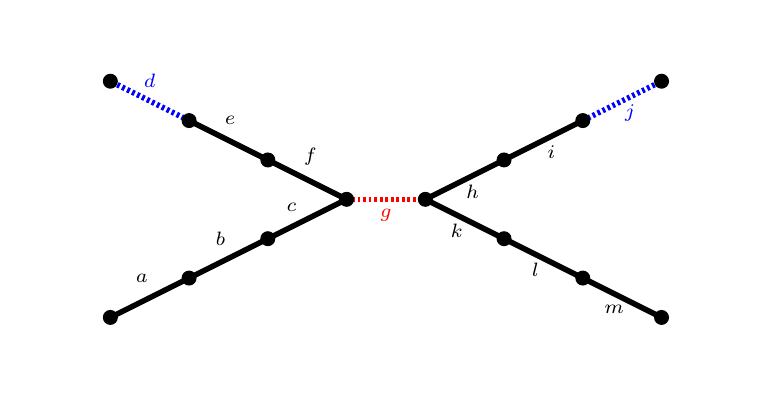
\begin{tikzpicture}[x=1cm,y=1cm]
\clip(-1.05,-2.24) rectangle (8,2.18);
\draw [line width=2pt,dash pattern=on 1pt off 1pt,color=red] (3,0)-- (4,0);
\draw [line width=2pt] (3,0)-- (2,0.5);
\draw [line width=2pt] (2,0.5)-- (1,1);
\draw [line width=2pt,dash pattern=on 1pt off 1pt,color=blue] (1,1)-- (0,1.5);
\draw [line width=2pt] (3,0)-- (2,-0.5);
\draw [line width=2pt] (2,-0.5)-- (1,-1);
\draw [line width=2pt] (1,-1)-- (0,-1.5);
\draw [line width=2pt] (4,0)-- (5,-0.5);
\draw [line width=2pt] (5,-0.5)-- (6,-1);
\draw [line width=2pt] (6,-1)-- (7,-1.5);
\draw [line width=2pt] (4,0)-- (5,0.5);
\draw [line width=2pt] (5,0.5)-- (6,1);
\draw [line width=2pt,dash pattern=on 1pt off 1pt,color=blue] (6,1)-- (7,1.5);
\begin{scriptsize}
\draw [fill=black] (3,0) circle (2.5pt);
\draw [fill=black] (4,0) circle (2.5pt);
\draw[color=red] (3.5,-0.2) node {$g$};
\draw [fill=black] (2,0.5) circle (2.5pt);
\draw[color=black] (2.54,0.54) node {$f$};
\draw [fill=black] (1,1) circle (2.5pt);
\draw[color=black] (1.52,1) node {$e$};
\draw [fill=black] (0,1.5) circle (2.5pt);
\draw[color=blue] (0.5,1.5) node {$d$};
\draw [fill=black] (2,-0.5) circle (2.5pt);
\draw[color=black] (2.3,-0.1) node {$c$};
\draw [fill=black] (1,-1) circle (2.5pt);
\draw[color=black] (1.4,-0.5) node {$b$};
\draw [fill=black] (0,-1.5) circle (2.5pt);
\draw[color=black] (0.4,-1) node {$a$};
\draw [fill=black] (5,-0.5) circle (2.5pt);
\draw[color=black] (4.4,-0.4) node {$k$};
\draw [fill=black] (6,-1) circle (2.5pt);
\draw[color=black] (5.4,-0.9) node {$l$};
\draw [fill=black] (7,-1.5) circle (2.5pt);
\draw[color=black] (6.4,-1.4) node {$m$};
\draw [fill=black] (5,0.5) circle (2.5pt);
\draw[color=black] (4.6,0.1) node {$h$};
\draw [fill=black] (6,1) circle (2.5pt);
\draw[color=black] (5.6,0.6) node {$i$};
\draw [fill=black] (7,1.5) circle (2.5pt);
\draw[color=blue] (6.6,1.1) node {$j$};
\end{scriptsize}
\end{tikzpicture}
\end{center}
 In the graph on the picture let $X=\{a,b,c,d,e,f,h,i,j,k,l,m\}=E\setminus\{g\}$ and $Y=E\setminus \{d,j\}$, thus $X;Y\in \mathcal F$ and $|X|=12>|Y|=11$. For all $x\in X\setminus Y=\{d,j\}$, $Y\cup \{x\}$ is not festive. Therefore $(E,\mathcal F)$ is not a matroid.

  \subsubsection*{(ii) There is no  set $J$ which is the edge set of a spanning christmas tree in both $G_1$ and $G_2$.}
  In  the graph $G_2$ every three edges of $\{e,f,g,h,i\}$ build a cycle, as a christmas tree has no cycles, we know $|J\cap \{e,f,g,h,i\}|\leq 2$. In graph $G_1$ the same is true for the set $\{a,b,c,d,j\}$ we get $|J\cap \{a,b,c,d,j\}|\leq 2$. Thus for $E=E(G_1)=E(G_2)$ it is $|J|=|J\cap E|=|J\cap \{a,b,c,d,j\}|+|J\cap \{e,f,g,h,i\}|\leq 4$, which is a contradiction to $J$ being a spanning tree, as both graphs have 6 vertices and thus we need $|J|=5$. Therefore statement (ii) is false.

\end{document}
